\documentclass{article}
\usepackage{csvsimple}
\usepackage{amsmath}
\usepackage{amssymb}
\usepackage{graphicx}
\usepackage{hyperref}
\usepackage{wrapfig}
\usepackage[utf8]{inputenc}
\usepackage{graphicx}
\usepackage[
backend=biber,
style=alphabetic,
]{biblatex}
\usepackage{multicol}
\usepackage{setspace}
\usepackage{datetime}
\usepackage{flushend} % For end of document
\usepackage[super]{nth}
\usepackage{enumitem} % to use custom enumration

% \addbibresource{rcheruiyotrefs.bib} %Imports bibliography file
\addbibresource{refs.bib}

\begin{document}

%insert your content here..

\section{Student content}
% added \usepackage[utf8]{inputenc} to Assignment3-git.tex
% added \usepackage{graphicx} to Assignment3-git.tex
% appended {IEEEtran} to \documentclass{article} in Assignment3-git.tex
% removed the \ { } characters surrounding KoraComments
% changed lines below
%  \bibliographystyle{IEEEtran}
%  \bibliography{refs}
% to \addbibresource{refs.bib} added to Assignment3-git.tex
% would include \printbibliography, however, I do not know what to cite for them
\section{Fall 2024 Student Content}

\documentclass{article}
\usepackage{graphicx} % Required for inserting images
\usepackage{fullpage}
\title{Thapa-F24}
\author{Sahil Thapa}
\date{October 2024}

\begin{document}

\maketitle

\section{Introduction: Sahil Thapa}
I am Sahil Thapa, a PhD in Computer Science. My advisor, Dr. Oluwatosin Oluwadare, guides my research, and I also serve as a graduate research assistant in his bioinformatics lab. My research focuses on utilizing deep learning and artificial intelligence to develop bioinformatics tools, with a current emphasis on splice site detection methods.\\

From a young age, I have enjoyed walking and traveling, a passion instilled in me by my maternal uncle. He often took me to rivers and hills, where we would sit and talk, fostering my love for trekking. I have explored many beautiful places in Nepal, including the Annapurna Mountain Range and the Langtang Circuit. My favorite films are "The Legend of 1900" and "The Forrest Gump."

\begin{figure}[h!]
    \centering
    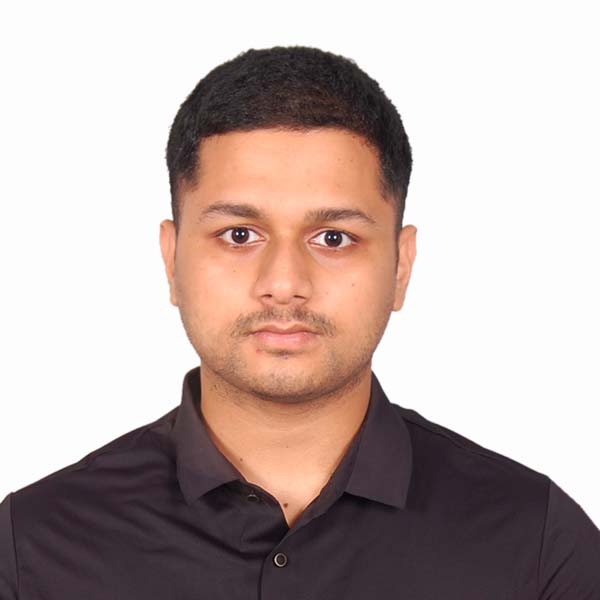
\includegraphics[width=0.5\linewidth]{Sahil_Thapa.jpg}
    \caption{Caption}
    \label{fig:enter-label}
\end{figure}

\section{Output of CNNSplice: Robust models for splice site prediction using convolutional neural networks.}
I explored the following Git repository related to my research: https://github.com/OluwadareLab/CNNSplice.git\\

CNNSplice is a set of deep convolutional neural network models designed for splice site prediction. Developed at the University of Colorado Colorado Springs, CNNSplice aims to efficiently predict true and false splice sites using robust machine learning techniques.

\subsection{test\_logfile\_metrics}
These are Output\_logfile Results of CNNModel.\\
$\{'precision': 0.9027834069851564, 'recall': 0.9206222222222222, 'f1': 0.9111579557303049, 'class_accuracy': 0.9318666666666666, 'accuracy': 0.9318666458129883\}$\\

$\{'precision': 0.9273229649052265, 'recall': 0.9525333333333332, 'f1': 0.9389124679859917, 'class_accuracy': 0.9528, 'accuracy': 0.9527999758720398\}$\\

$\{'precision': 0.9229379328722263, 'recall': 0.9288888888888889, 'f1': 0.925857755161124, 'class_accuracy': 0.944, 'accuracy': 0.9440000057220459\}$\\

$\{'precision': 0.9280761354666826, 'recall': 0.9274666666666667, 'f1': 0.927770831864634, 'class_accuracy': 0.9458666666666666, 'accuracy': 0.9458666443824768\}$\\

$\{'precision': 0.9037206096479873, 'recall': 0.9141333333333334, 'f1': 0.908744230763471, 'class_accuracy': 0.9306666666666666, 'accuracy': 0.9306666851043701\}$

\begin{figure}[h!]
    \centering
    \includegraphics[width=0.5\linewidth]{LogFile.png}
    \caption{LogFile}
    \label{fig:enter-label}
\end{figure}


\section{Questions for me:}


\end{document}

\subsection{Raja Kantheti}
I am a master's student in Computer Science at UCCS. I want to choose the thesis path to satisfy the degree requirements. My expected course outcomes are to learn what it means to conduct research, how to write scientific papers, better articulate my ideas and evaluate their novelty, and write at least one paper of any type by the end of the semester.

I want to do my thesis on processor pipeline design, which would optimize branch prediction using additional prefetching and decoding units in parallel with the central decode unit. This pipeline could also mitigate SPECTRE attacks, which exploit Speculative execution. 

I am determined to evaluate my thesis proposal, understand the necessary steps to evaluate the outcomes of my thesis, and grasp the elements of a successful proposal. I am also excited to challenge myself, to see if I have the stamina for long-term research and if this path is the right one for my career progression.

Some personal things about me outside of academia are that I like to be in solitude from time to time, lost in my thoughts and devices, contemplating meta-ethics, talking and debating with myself, and exploring all possibilities. The routines that would allow me to do this are my hobbies: Long walks and longer drives, camping alone, hiking in state/national parks and, wood carving. 
\begin{figure}[h]
\centering
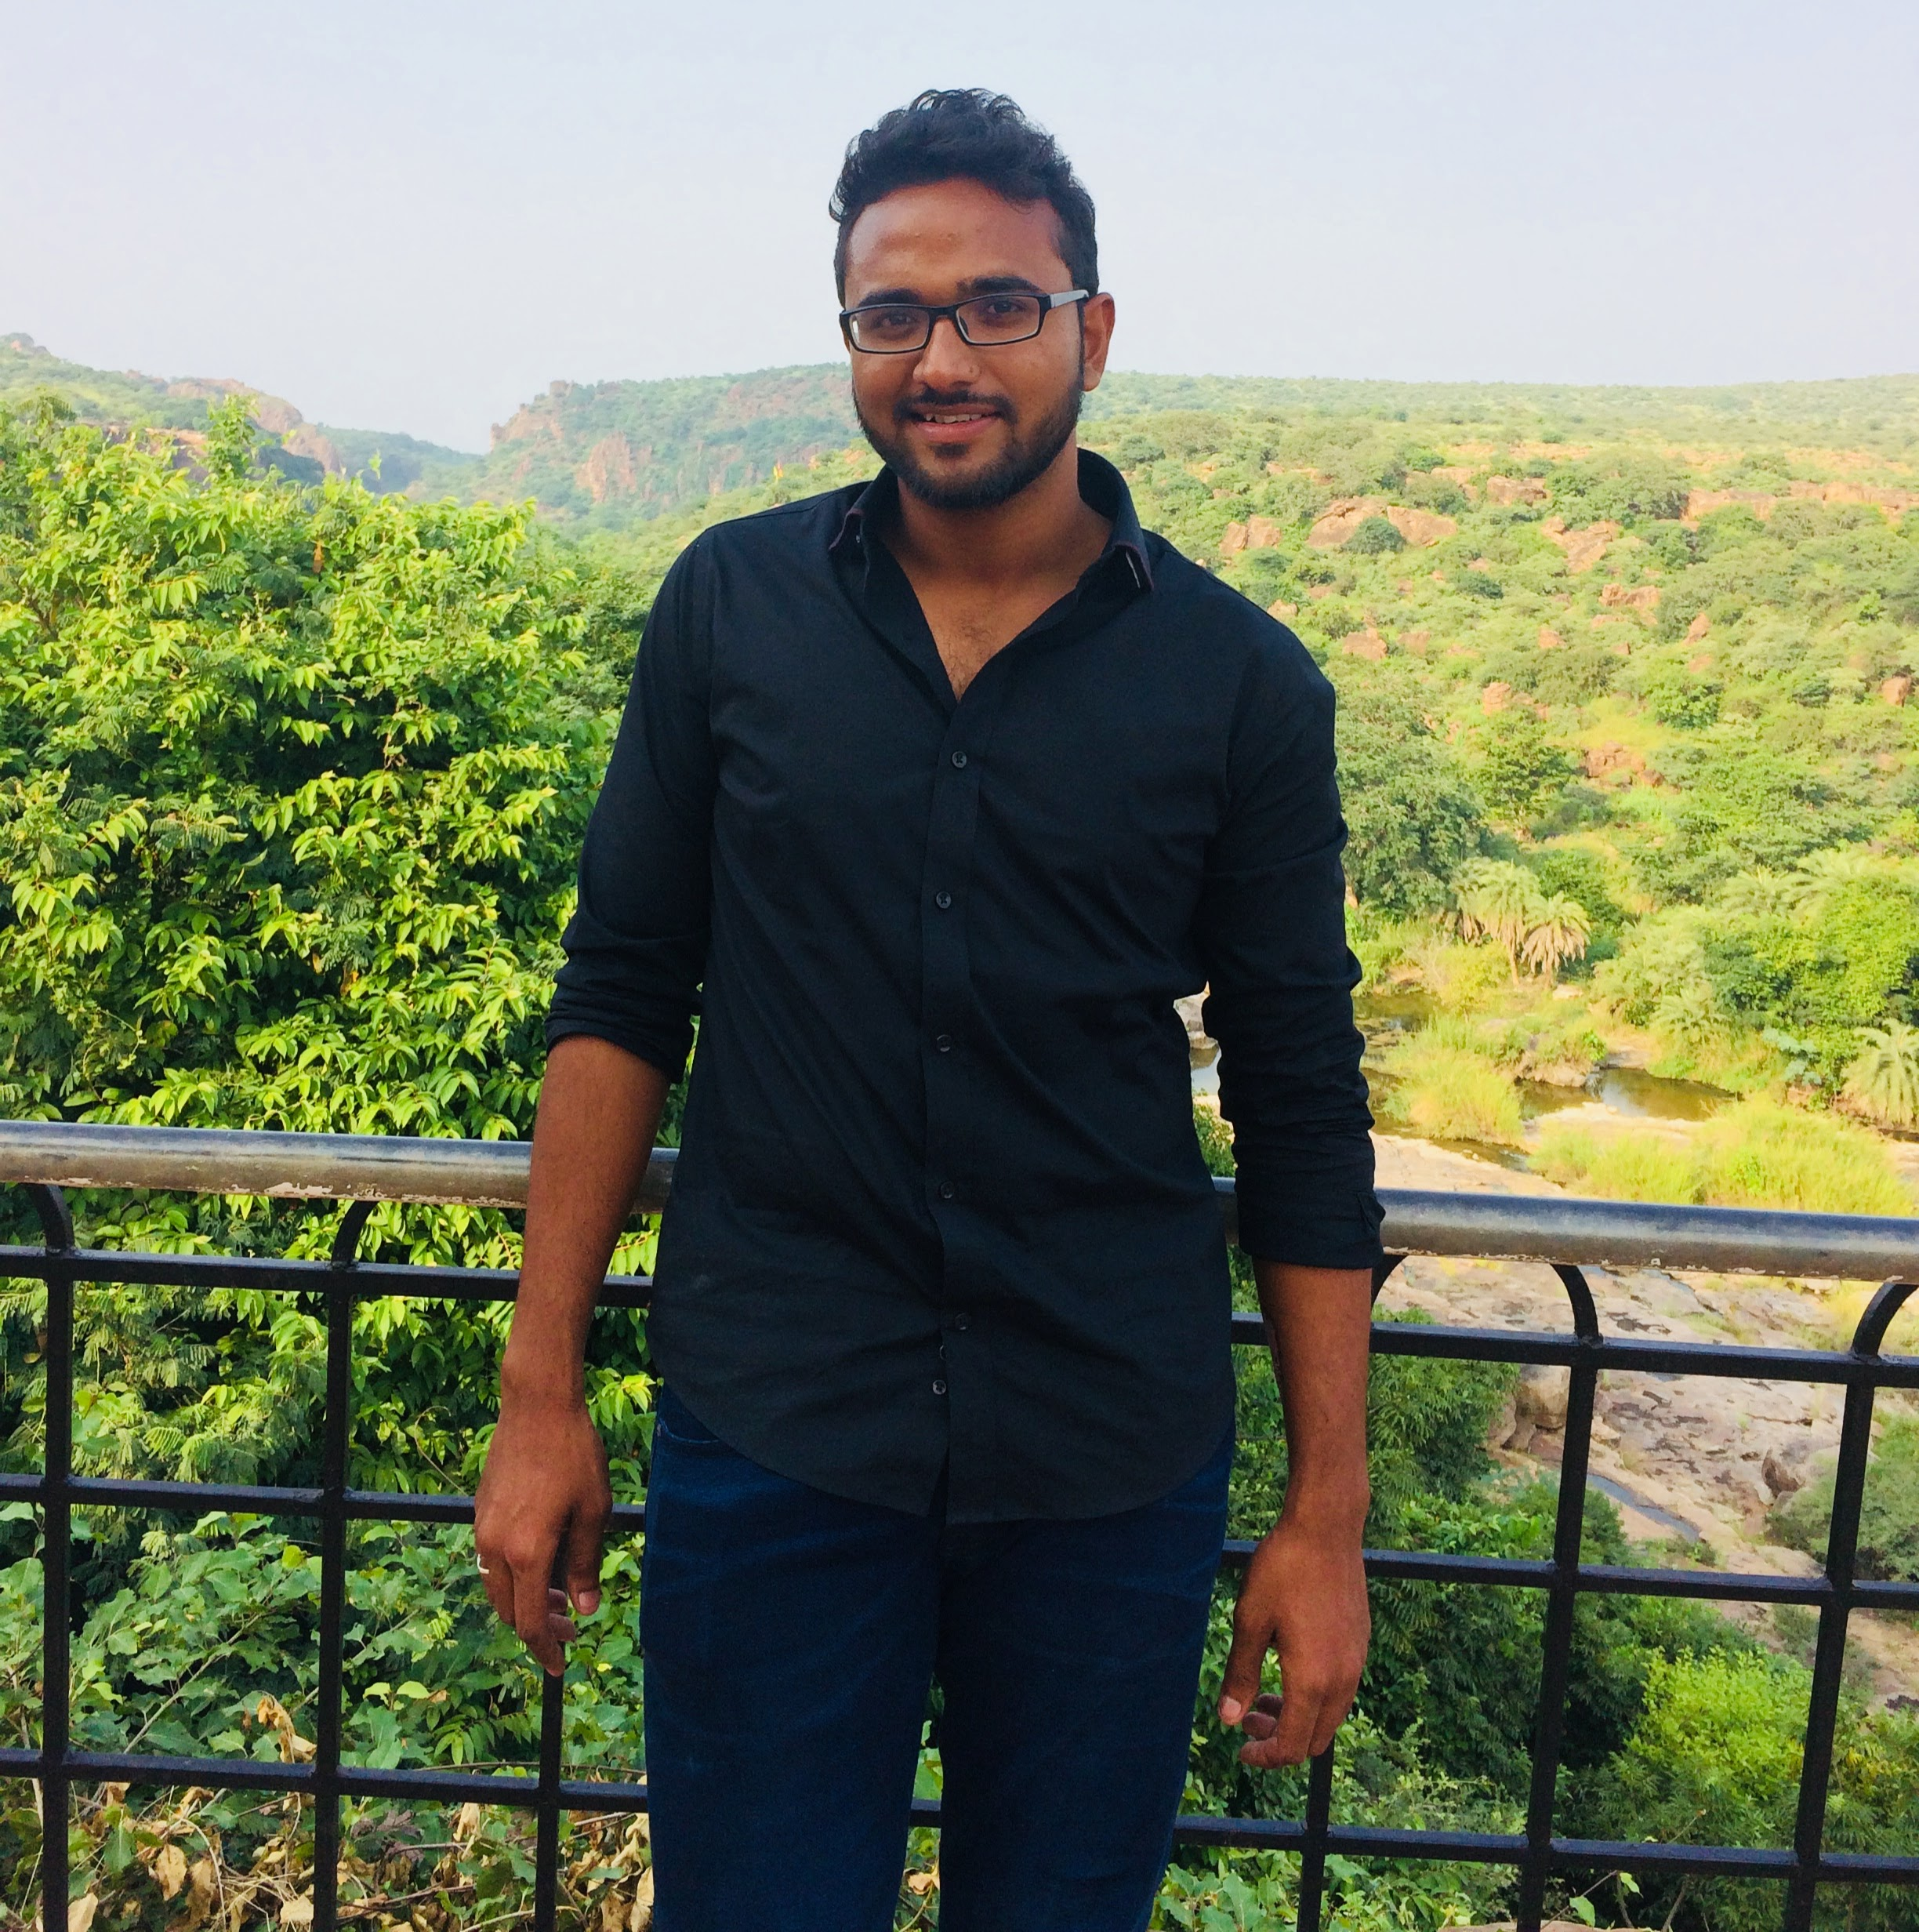
\includegraphics[width=0.25\linewidth]{images/IMG_1667.JPG}
\caption{'tis I. }
\end{figure}

\section*{Output of the gem5 simulator: Running a test program: }
gem5 is a cycle accurate simulator widely used in Computer Architecture Research. 
It is used to simulate the behavior of a computer system. 
The output of the gem5 simulator is a trace of the instructions executed by the processor. 
The trace is a list of instructions executed by the processor, along with the cycle number at which the instruction was executed.
The trace can be used to analyze the performance of the processor, and to identify bottlenecks in the processor design.

The simulation will produce a file with numerous metrics below are some of the metrics used by me for the survey paper.\\
This is a simulation for risc-v ISA on a MINOR CPU for a  likedlist program. 

simSeconds      0.001541 \# Number of seconds simulated (Second)\\
simTicks      1540878200 \# Number of ticks simulated (Tick)\\
finalTick     1540878200 \# Number of ticks from beginning of \\simulation (restored from checkpoints and never reset) (Tick)\\
simFreq     1000000000000 \# The number of ticks per simulated second ((Tick/Second))\\
hostSeconds         0.22 \# Real time elapsed on the host (Second)\\
hostTickRate  6962621095 \# The number of ticks simulated per host second (ticks/s) ((Tick/Second))\\
hostMemory       1158876 \# Number of bytes of host memory used (Byte)\\
simInsts          113770 \# Number of instructions simulated (Count)\\
simOps            113776 \# Number of ops (including micro ops) simulated (Count)\\
hostInstRate      513943 \# Simulator instruction rate (inst/s) ((Count/Second))\\
hostOpRate        513963 \# Simulator op (including micro ops) rate (op/s) ((Count/Second))\\
board.processor.cores0.core.branchPred.lookups        29946 \# Number of BP lookups (Count)\\
board.processor.cores0.core.branchPred.condPredicted  21139 \# Number of conditional branches predicted (Count)\\
board.processor.cores0.core.branchPred.condIncorrect  462 \# Number of conditional branches incorrect (Count)\\
board.processor.cores0.core.branchPred.BTBLookups     10899 \# Number of BTB lookups (Count)\\
board.processor.cores0.core.branchPred.BTBUpdates     396 \# Number of BTB updates (Count)\\
board.processor.cores0.core.branchPred.BTBHits        10187 \# Number of BTB hits (Count)\\
board.processor.cores0.core.branchPred.BTBHitRatio    0.934673 \# BTB Hit Ratio (Ratio)\\
board.processor.cores0.core.branchPred.RASUsed         2019 \# Number of times the RAS was used to get a target. (Count)\\
board.processor.cores0.core.branchPred.RASIncorrect     5 \# Number of incorrect RAS predictions. (Count)\\
board.processor.cores0.core.branchPred.indirectLookups  1790 \# Number of indirect predictor lookups. (Count)\\
board.processor.cores0.core.branchPred.indirectHits     1748 \# Number of indirect target hits. (Count)\\
board.processor.cores0.core.branchPred.indirectMisses    42 \# Number of indirect misses. (Count)\\
board.processor.cores0.core.branchPred.indirectMispredicted  24 \# Number of mispredicted indirect branches. (Count)\\

\section*{Questions For me: }
Your work looks interesting from a computer architecture perspective. However, you have mentioned that it is based on risc-v architecture, in the current context, how is the scenario of this architecture being used in real world applications? What do you see the future prospects of it? 
\section{Goals for the Course}

As a PhD candidate in Security under the guidance of Dr Sang-Yoon Chang, my primary goal in the "Computer Science Research - CS 6000" course is to deepen my understanding of advanced research methodologies and refine my ability to conduct impactful research in security. This course represents a pivotal opportunity to explore the latest trends, challenges, and innovations in cybersecurity, allowing me to develop a comprehensive framework for addressing complex issues in this domain. Through rigorous analysis and the application of various research techniques, I aim to contribute novel insights to the academic community while also developing practical solutions that can be applied in real-world scenarios.\\

In particular, I am eager to enhance my skills in identifying, analyzing, and solving complex security problems, focusing on areas such as adversarial attacks, secure system design, and the development of robust defence mechanisms. By the end of this course, I hope to have a well-rounded understanding of how to conduct high-quality research that not only advances theoretical knowledge but also has tangible impacts on the security landscape. My ultimate goal is to leverage this knowledge to produce a dissertation that is both academically rigorous and practically significant, contributing to the field of cybersecurity in meaningful ways.\\

Personally, I am married and the father of two energetic boys, both seven years old. Balancing family life with academic pursuits is both challenging and rewarding, and I find that travelling with my family during free time and vacations provides the perfect opportunity to relax and gain new perspectives. My journey from Bangladesh to my current PhD program represents not just a professional ambition but also a personal commitment to growth and learning.

\begin{figure}[h!]
\centering
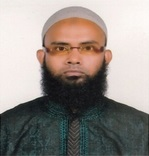
\includegraphics[width=0.5\textwidth]{images/Amanul_Islam.jpg}
\caption{Amanul Islam}
\label{fig:myphoto}
\end{figure}


\section*{Output of the Training and Validation Loss of Anomaly-Detection-in-Fake-Base-Station-using-Autoencoder: }

I tested the (https://github.com/Luckyaman/Anomaly-Detection-in-Fake-Base-Station-using-Autoencoder.git) related to anomaly detection in 5G networks.

For this project, I tested an autoencoder-based anomaly detection model for 5G networks using a GitHub repository. Over the course of 50 epochs, the model's training and validation losses converged, though fluctuating near similar values. The training process was time-intensive, with some epochs taking over two minutes each. Despite stable loss values, the model ultimately detected 717 anomalies from the dataset. The experience highlighted the need for careful tuning of hyperparameters and further exploration of feature engineering to improve the model’s performance. It was a valuable learning experience in anomaly detection within telecommunications networks.

Epoch 1/50
59902/59902 ━━━━━━━━━━━━━━━━━━━━ 120s 2ms/step - loss: 0.7488 - val_loss: 0.7521
Epoch 2/50
59902/59902 ━━━━━━━━━━━━━━━━━━━━ 115s 2ms/step - loss: 0.7974 - val_loss: 0.7516
Epoch 3/50
59902/59902 ━━━━━━━━━━━━━━━━━━━━ 122s 2ms/step - loss: 0.6965 - val_loss: 0.7520
Epoch 4/50
59902/59902 ━━━━━━━━━━━━━━━━━━━━ 124s 2ms/step - loss: 0.8732 - val_loss: 0.7520
Epoch 5/50
59902/59902 ━━━━━━━━━━━━━━━━━━━━ 129s 2ms/step - loss: 0.7421 - val_loss: 0.7518
Epoch 6/50
59902/59902 ━━━━━━━━━━━━━━━━━━━━ 128s 2ms/step - loss: 0.9766 - val_loss: 0.7513
Epoch 7/50
59902/59902 ━━━━━━━━━━━━━━━━━━━━ 136s 2ms/step - loss: 0.7514 - val_loss: 0.7513
Epoch 8/50
59902/59902 ━━━━━━━━━━━━━━━━━━━━ 125s 2ms/step - loss: 0.9412 - val_loss: 0.7512
Epoch 9/50
59902/59902 ━━━━━━━━━━━━━━━━━━━━ 126s 2ms/step - loss: 0.7056 - val_loss: 0.7512
Epoch 10/50
59902/59902 ━━━━━━━━━━━━━━━━━━━━ 145s 2ms/step - loss: 0.8189 - val_loss: 0.7518
Epoch 11/50
59902/59902 ━━━━━━━━━━━━━━━━━━━━ 134s 2ms/step - loss: 0.8691 - val_loss: 0.7512
Epoch 12/50
59902/59902 ━━━━━━━━━━━━━━━━━━━━ 121s 2ms/step - loss: 0.7325 - val_loss: 0.7512
Epoch 13/50
59902/59902 ━━━━━━━━━━━━━━━━━━━━ 120s 2ms/step - loss: 0.7405 - val_loss: 0.7519
Epoch 14/50
59902/59902 ━━━━━━━━━━━━━━━━━━━━ 124s 2ms/step - loss: 0.8846 - val_loss: 0.7517
Epoch 15/50
59902/59902 ━━━━━━━━━━━━━━━━━━━━ 166s 2ms/step - loss: 0.8146 - val_loss: 0.7517
Epoch 16/50
59902/59902 ━━━━━━━━━━━━━━━━━━━━ 191s 2ms/step - loss: 0.8228 - val_loss: 0.7512
Epoch 17/50
59902/59902 ━━━━━━━━━━━━━━━━━━━━ 148s 2ms/step - loss: 0.8338 - val_loss: 0.7512
Epoch 18/50
59902/59902 ━━━━━━━━━━━━━━━━━━━━ 219s 3ms/step - loss: 0.9288 - val_loss: 0.7512
Epoch 19/50
59902/59902 ━━━━━━━━━━━━━━━━━━━━ 182s 2ms/step - loss: 0.8441 - val_loss: 0.7512
Epoch 20/50
59902/59902 ━━━━━━━━━━━━━━━━━━━━ 127s 2ms/step - loss: 0.8198 - val_loss: 0.7512
Epoch 21/50
59902/59902 ━━━━━━━━━━━━━━━━━━━━ 126s 2ms/step - loss: 0.7595 - val_loss: 0.7516
Epoch 22/50
59902/59902 ━━━━━━━━━━━━━━━━━━━━ 139s 2ms/step - loss: 0.9608 - val_loss: 0.7518
Epoch 23/50
59902/59902 ━━━━━━━━━━━━━━━━━━━━ 122s 2ms/step - loss: 0.8043 - val_loss: 0.7512
Epoch 24/50
59902/59902 ━━━━━━━━━━━━━━━━━━━━ 144s 2ms/step - loss: 0.8094 - val_loss: 0.7523
Epoch 25/50
59902/59902 ━━━━━━━━━━━━━━━━━━━━ 143s 2ms/step - loss: 0.8531 - val_loss: 0.7512
Epoch 26/50
59902/59902 ━━━━━━━━━━━━━━━━━━━━ 121s 2ms/step - loss: 0.7947 - val_loss: 0.7511
Epoch 27/50
59902/59902 ━━━━━━━━━━━━━━━━━━━━ 123s 2ms/step - loss: 0.7315 - val_loss: 0.7512
Epoch 28/50
59902/59902 ━━━━━━━━━━━━━━━━━━━━ 122s 2ms/step - loss: 0.8460 - val_loss: 0.7512
Epoch 29/50
59902/59902 ━━━━━━━━━━━━━━━━━━━━ 116s 2ms/step - loss: 0.7275 - val_loss: 0.7517
Epoch 30/50
59902/59902 ━━━━━━━━━━━━━━━━━━━━ 137s 2ms/step - loss: 0.8481 - val_loss: 0.7512
Epoch 31/50
59902/59902 ━━━━━━━━━━━━━━━━━━━━ 144s 2ms/step - loss: 0.8883 - val_loss: 0.7512
Epoch 32/50
59902/59902 ━━━━━━━━━━━━━━━━━━━━ 111s 2ms/step - loss: 0.9098 - val_loss: 0.7512
Epoch 33/50
59902/59902 ━━━━━━━━━━━━━━━━━━━━ 111s 2ms/step - loss: 0.8350 - val_loss: 0.7512
Epoch 34/50
59902/59902 ━━━━━━━━━━━━━━━━━━━━ 145s 2ms/step - loss: 0.7062 - val_loss: 0.7512
Epoch 35/50
59902/59902 ━━━━━━━━━━━━━━━━━━━━ 139s 2ms/step - loss: 0.8112 - val_loss: 0.7511
Epoch 36/50
59902/59902 ━━━━━━━━━━━━━━━━━━━━ 152s 2ms/step - loss: 1.0590 - val_loss: 0.7513
Epoch 37/50
59902/59902 ━━━━━━━━━━━━━━━━━━━━ 123s 2ms/step - loss: 0.7585 - val_loss: 0.7512
Epoch 38/50
59902/59902 ━━━━━━━━━━━━━━━━━━━━ 139s 2ms/step - loss: 0.7457 - val_loss: 0.7517
Epoch 39/50
59902/59902 ━━━━━━━━━━━━━━━━━━━━ 136s 2ms/step - loss: 0.7591 - val_loss: 0.7517
Epoch 40/50
59902/59902 ━━━━━━━━━━━━━━━━━━━━ 134s 2ms/step - loss: 0.7131 - val_loss: 0.7512
Epoch 41/50
59902/59902 ━━━━━━━━━━━━━━━━━━━━ 143s 2ms/step - loss: 0.8032 - val_loss: 0.7511
Epoch 42/50
59902/59902 ━━━━━━━━━━━━━━━━━━━━ 133s 2ms/step - loss: 0.7928 - val_loss: 0.7512
Epoch 43/50
59902/59902 ━━━━━━━━━━━━━━━━━━━━ 150s 2ms/step - loss: 0.8165 - val_loss: 0.7512
Epoch 44/50
59902/59902 ━━━━━━━━━━━━━━━━━━━━ 136s 2ms/step - loss: 1.1533 - val_loss: 0.7517
Epoch 45/50
59902/59902 ━━━━━━━━━━━━━━━━━━━━ 148s 2ms/step - loss: 0.7264 - val_loss: 0.7512
Epoch 46/50
59902/59902 ━━━━━━━━━━━━━━━━━━━━ 141s 2ms/step - loss: 0.8815 - val_loss: 0.7511
Epoch 47/50
59902/59902 ━━━━━━━━━━━━━━━━━━━━ 146s 2ms/step - loss: 0.7979 - val_loss: 0.7514
Epoch 48/50
59902/59902 ━━━━━━━━━━━━━━━━━━━━ 211s 3ms/step - loss: 0.8380 - val_loss: 0.7511
Epoch 49/50
59902/59902 ━━━━━━━━━━━━━━━━━━━━ 152s 3ms/step - loss: 0.7694 - val_loss: 0.7511
Epoch 50/50
59902/59902 ━━━━━━━━━━━━━━━━━━━━ 200s 3ms/step - loss: 0.7637 - val_loss: 0.7511
74877/74877 ━━━━━━━━━━━━━━━━━━━━ 130s 2ms/step
Number of anomalies detected: 717

\section*{Questions: }

%created "images" directory in the repo. 
\section{Marwan Alharbi}

This is my content

\section{Example of Easy Tables}
\csvautotabular{test.csv}


\section*{Better formated Tables}
    \begin{tabular}{r|r|r}%
    % specify table head
    \bf Time (s) & \bf Rel. time (s)& \bf Y Pos
% use head of csv as column names
    \csvreader{test.csv}{}
% specify selected coloumns here
    {\\\hline\csvcoli&\csvcolii&\csvcolvi}
    \end{tabular}
    \clearpage


\end{document}
